\documentclass[letterpaper,12pt]{article}
\usepackage[margin=1in]{geometry}
\usepackage{graphicx}  % Include figure files
\usepackage{xcolor}  % Allow for a color text
\usepackage{amsmath}  % math fonts
\usepackage{amsfonts}  % math fonts
\usepackage{latexsym}  % math fonts
\usepackage{amssymb}  % math fonts
\usepackage{mathtools} % Give more control of how equations are displayed
\usepackage{appendix} % Lets you create an appendix
\usepackage[numbered]{matlab-prettifier} % Let's me import MATLAB code in a nice format
\usepackage{indentfirst} % This indents the first paragraph. By default latex won't do it.
\usepackage{subfigure}

\setlength{\parskip}{1em} % This skips a line when making new paragraphs
\newtagform{show_eq}{(Eq.\ }{)}  % how the equation numbers are displayed
\usetagform{show_eq} % this goes with the \newtagform

\begin{document}

% ================================== Title Page ==========================================
\begin{titlepage}
 \begin{center}
 \vspace*{1in}
{\Huge Digital Signal Processing and Analysis of Signals in the Power Spectrum}\\
    \bigskip
    by\\
    \bigskip
    {\Large Kevin Moran} \\
    \bigskip
    Lab Partner : Cade Hermeston\\
    Date of Experiment : Thursday, October 29th, 2020

    \bigskip\bigskip\bigskip
    University of Southern California\\
    Aerospace and Mechanical Engineering Department\\
    AME 341A : Mechoptronics
 \end{center}
\end{titlepage}

% ----------------------- Abstract ------------------------------------
\begin{abstract}
    Utilizing the power spectra for digital signal processing provides a efficient method for managing, interpreting, and transmitting data. By using a function generator to control various types of signals and a National Instruments data acquisition system with a custom virtual interface to collect data, signals were successfully measured and represented in the frequency domain. Using a sampling rate of 2500 Hz, a sine wave with frequency of 1500 Hz was purposely aliased and represented in the power spectrum with an observable frequency of 1001 Hz. Additionally, an unknown signal was replicated by analyzing fundamental frequencies and harmonics in the power spectrum. This unknown signal was determined to be comprised of a 777 Hz sine wave embedded in a 33 Hz triangle wave with 50\% symmetry.   
\end{abstract}

% ------------------------- Main Text ----------------------------------
\section{Introduction}
Digital Signal Processing (DSP) is essential to making digital measurements of real-world signals, and components such as an analog to digital converter (ADC) allows for the measurement of natural signals via electronic devices. Furthermore, DSP is essential for communication applications and is a fundamental component of data acquisition systems found throughout almost every area of engineering. Processing, filtering, and transmitting an enormous amount of data as a time trace of voltage, however, is extremely difficult due to limitations set by computing power. Continuous signals can be transformed into a power spectrum via Fourier transformation, thus making data easier to manage. For example, a sine wave of an AC current can be represented by a large set of data depending on the sampling frequency and number of data point or duration of the measurement or, this information can be represented in the power spectrum as a single point. The compact-ability of the signal simplifies data management and the information can be more easily transmitted, relative to the signal in the time domain. 

\subsection{Fourier Transformations}
As mentioned, the relationship between the frequency and time domain can be described by a Fourier transformation,
\begin{equation}
    y(t) = A_0 + \sum_{n=1}^\infty A_ncos(nwt) + B_nsin(nwt)
    \label{FourierEq}
\end{equation}
where $w$ and $t$ represent the natural frequency and time, respectively. The variable $n$ represents the harmonics associated with the signal and the special case where $n=1$ is known as the fundamental frequency. The variables $A_0, \ A_n$, and $B_n$ can be expressed as the subset of equations
\begin{gather*}
    A_0 = \frac{1}{T} \int_{-T/2}^{T/2} y(t)\ dt \\
    A_n = \frac{2}{T} \int_{-T/2}^{T/2} y(t)cos(nwt)\ dt \\
    B_n = \frac{1}{T} \int_{-T/2}^{T/2} y(t)sin(nwt)\ dt 
\end{gather*}
where $T$ is the period of the signal and $A_0$ is often referred to as the offset of a signal. The purpose of a Fourier transformation is to represent a continuous function as an infinite sum and, in the case of square and triangle waves, the systems harmonics. 

In the scope of this paper, the Fourier transformation of a square wave can be described as 
\begin{equation}
    y(t) = \sum_{n=1,3,5...}^\infty \frac{4}{n\pi}sin(nwt)
    \label{squareFourierEq}
\end{equation}
and is strictly in terms of odd harmonics. Similarly, the Fourier transformation of a triangle wave can be described by the equation
\begin{equation}
    y(t) = \sum_{n=1,3,5...}^\infty \frac{8}{n^2\pi^2}cos(nwt)
    \label{triangleFourierEq}
\end{equation}

\subsection{Nyquist Frequency}
The Nyquist Frequency, defined by the relationship
\begin{equation}
    f_{Ny} = \frac{f_s}{2}
    \label{NyFreqEq}
\end{equation}
is the largest observable frequency that can be measured before aliasing occurs. Attempting to resolve any signal beyond the Nyquist frequency in the time domain will result in a loss of shape, amplitude, and \emph{folds back}, on itself in the power spectrum. If a signal is aliased, the observable frequency can be represented as

\begin{equation}
    f_{obs} = f_s - f
    \label{fobsEq}
\end{equation}
where $f_s$ and $f$ represent the sampling frequency and frequency of the signal. 

% ---------------------------- M & M --------------------------------------- 


\section{Methods and Materials}
By using a National Instrument VirtualBench VB-8012 (VBench) to control input signals and a National Instrument data acquisition (NI-DAQ) system with a custom virtual interface to collect data, various signals were processed in the frequency and time domain. The experiment focused on three primary modes; analyzing a well known signal in the frequency domain, examining the response for a signal being aliased in the frequency domain and time domain, and determining the characteristics of an unknown signal in the frequency and time domain.

\subsection{Power Spectrum Representation}
To establish a foundational understanding for interpreting signals in the frequency domain, the VBench function generator was used to create a sine and square wave. Both of these signals were created using the parameters, 2 $V_{rms}$ amplitude and a frequency of 100 Hz. For the sine wave, a sampling rate of 400Hz was chosen to ensure the no aliasing of the signal occurred. Collecting enough data for the square wave, however, required a higher sampling frequency of 10 kHz due to the harmonics expressed in Equation \ref{squareFourierEq}.

\subsection{Aliasing of a Known Signal}
To properly demonstrate the \emph{fold back} type of behavior associated with aliasing a sine wave requires a non-aliased measurement for comparison. Therefore a sampling frequency of 10 kHz was chosen to measure a 1500 Hz signal. This ensured that the frequency of the signal was well below the Nyquist frequency described in Equation \ref{NyFreqEq}. Additionally, the same signal was also analyzed using a sampling frequency of 2.5 kHz. These two sampling frequencies ensured that data was collected under aliased and non-aliased conditions.

To further analyze a sine wave under aliasing conditions, the signal was analyzed in the time domain of the virtual interface using sampling frequencies of 2.5 kHz and 1.5 kHz. To conclude the experimental observations of an aliased sine wave in the time domain, the frequency of the signal was changed in increments of 1 Hz on the interval from 1,500 Hz to 1,510 Hz.

\subsection{Characterizing an Unknown Signal}
Characterizing the unknown signal was accomplished by setting the sampling rate to 20 kHz and examining the time trace for continuity and a well defined shaped, thus ensuring the signal was not being aliased. Afterwards, the sampling frequency was set to 2,000 kHz and then 1,000 kHz, and data sets were collected using the NI-DAQ in the frequency domain for both sampling frequencies.   

\section{Results and Discussion} % ::::::::::::::::::::::::::::::::::::::::::::::::::::::::::::::::::::::::::::::::::::::::::::::::::::::::::::::

\subsection{Analysis of Known Signal} 

Figure 1 shows the results for sine and square waves generated with the VBench in the frequency domain. Both signals satisfy the condition $f_s > f_{Ny}$ and thus ensure no aliasing is occurring. Furthermore, the fundamental frequency in Figure \ref{sin} corresponds to the same frequency on the function generator and the harmonic frequencies in Figure \ref{square} match the values associated with the Fourier transformation expressed in the Equation \ref{squareFourierEq} (i.e., $3f,\ 5f,\ 7f,...)$.  

% :::::::::::::::::: Sine and Square Wave Subsection ::::::::::::::::::
\begin{figure}[ht]
\centering
\subfigure[Sine Wave]{
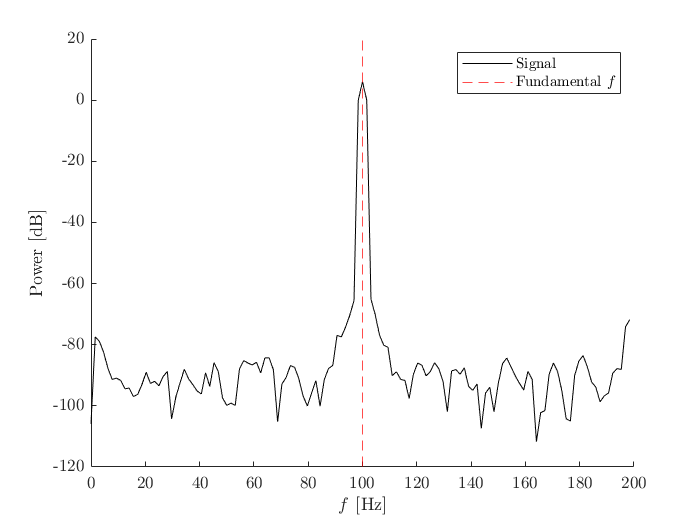
\includegraphics[width=.4\linewidth]{sin.png}
\label{sin}}
\quad
\subfigure[Square Wave]{
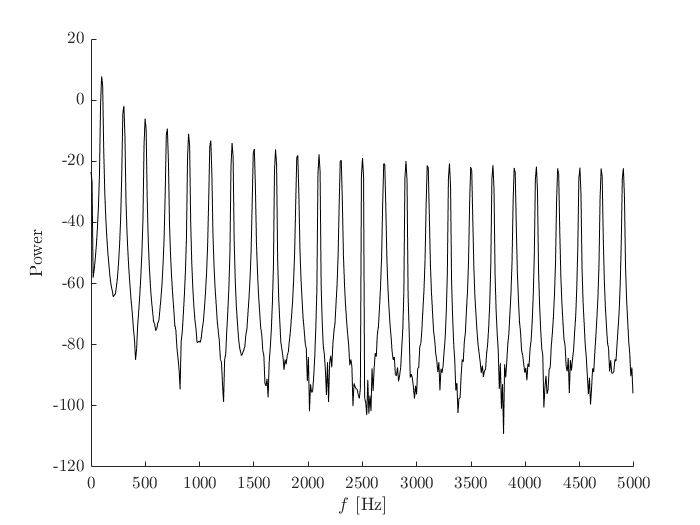
\includegraphics[width=.4\linewidth]{square.png}
\label{square}}
\caption{Sine and square waves with $V_{rms}$ of 2 V at 100Hz shown in the frequency domain. Both of the signals are measured under non-aliasing conditions}
\label{Part1Images}
\end{figure}

Examining key characteristics of graphs shown in Figure \ref{Part1Images} and Figure \ref{Part2FreqDomain} reveals an agreement between theoretical predictions and experimental results for signals represented on a power spectra. In either case, signals generated via the VBench function generator were shown to have either single peaks or harmonics for sine and square waves, respectively. Table \ref{knownSignalTable} represents key values for graphs in Figure \ref{Part1Images}.

\begin{table}[ht]
    \centering
    \begin{tabular}{c|c||c|c|c|c}
         & Sine $f$ & Square $f$ & Square $f_3$ & Square $f_5$ & Square $f_7$ \\ \hline
         $f_{exp}$ [Hz] & 100  & 98  & 303 & 498 & 703\\ \hline
         $f_{theo}$ [Hz] & 100 & 100 & 300 & 500 & 700\\ \hline
         Power [dB] & 6 & 8 & -2 & -6 & -9
    \end{tabular}
    \caption{Caption}
    \label{knownSignalTable}
\end{table}

\subsection{Aliasing}
% :::::::::::::::::: Aliasing Subsection ::::::::::::::::::
On the contrary, Figure \ref{Part2FreqDomain} shows a 1.5 kHz sine wave purposely being aliased by setting the sampling frequency to 10 kHz, then reducing it to 2.5 kHz. Since the Nyquis frequency of the latter is less than the frequency of the signal, the observed frequency is expressed by Equation \ref{fobsEq} and illustrates the \emph{fold back} type of behavior expected in a aliased signal.

\begin{figure}[ht]
\centering
\subfigure[$f_s$ = 10 kHz]{
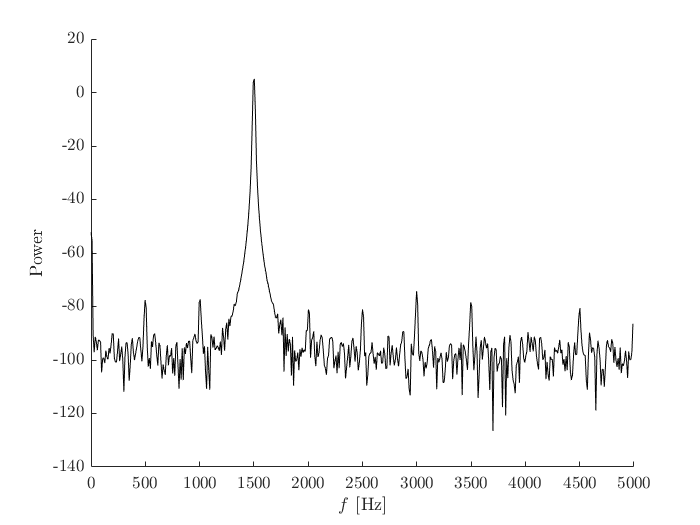
\includegraphics[width=.4\linewidth]{sin10000.png}
\label{NonAlisased}}
\quad
\subfigure[$f_s$ = 2.5 kHz]{
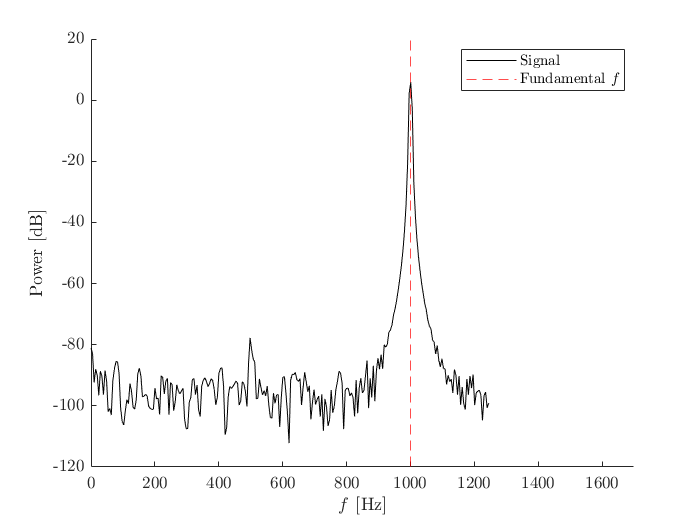
\includegraphics[width=.4\linewidth]{sine2500.png}
\label{Alisased}}
\caption{Demonstration of aliasing the frequency domain, where (a) and (b) are non-aliased and aliased signals, respectively. As per Equation \ref{NyFreqEq}, the $f_Ny$ for (a) and (b) are 5 kHz and 1.25 KHz, and the observed frequency of (b) is describe by Equation \ref{fobsEq} with a value of 1001 kHz.}
\label{Part2FreqDomain}
\end{figure}

Figure \ref{TimeDomainImages} illustrates the same signal in the time domain. This analysis indicated that using a sampling frequency of 2.5 kHz is not sufficient enough to return the amplitude nor shape of the signal, rather it only returns the frequency. Furthermore, Figure \ref{fs=f} illustrates the scenario $ f_s = f_{signal}$. In this situation, the sampling rate is no longer sufficient enough to collect any sort of data from the signal (i.e., shape, offset, frequency, or amplitude). However, incrementally increasing the frequency at the function generator, as shown in Figure \ref{fs<f}, seemed to restore the characteristics of the graph in the time domain. 

\begin{figure}[ht]
\centering
\subfigure[$f_s\ > \ f$]{
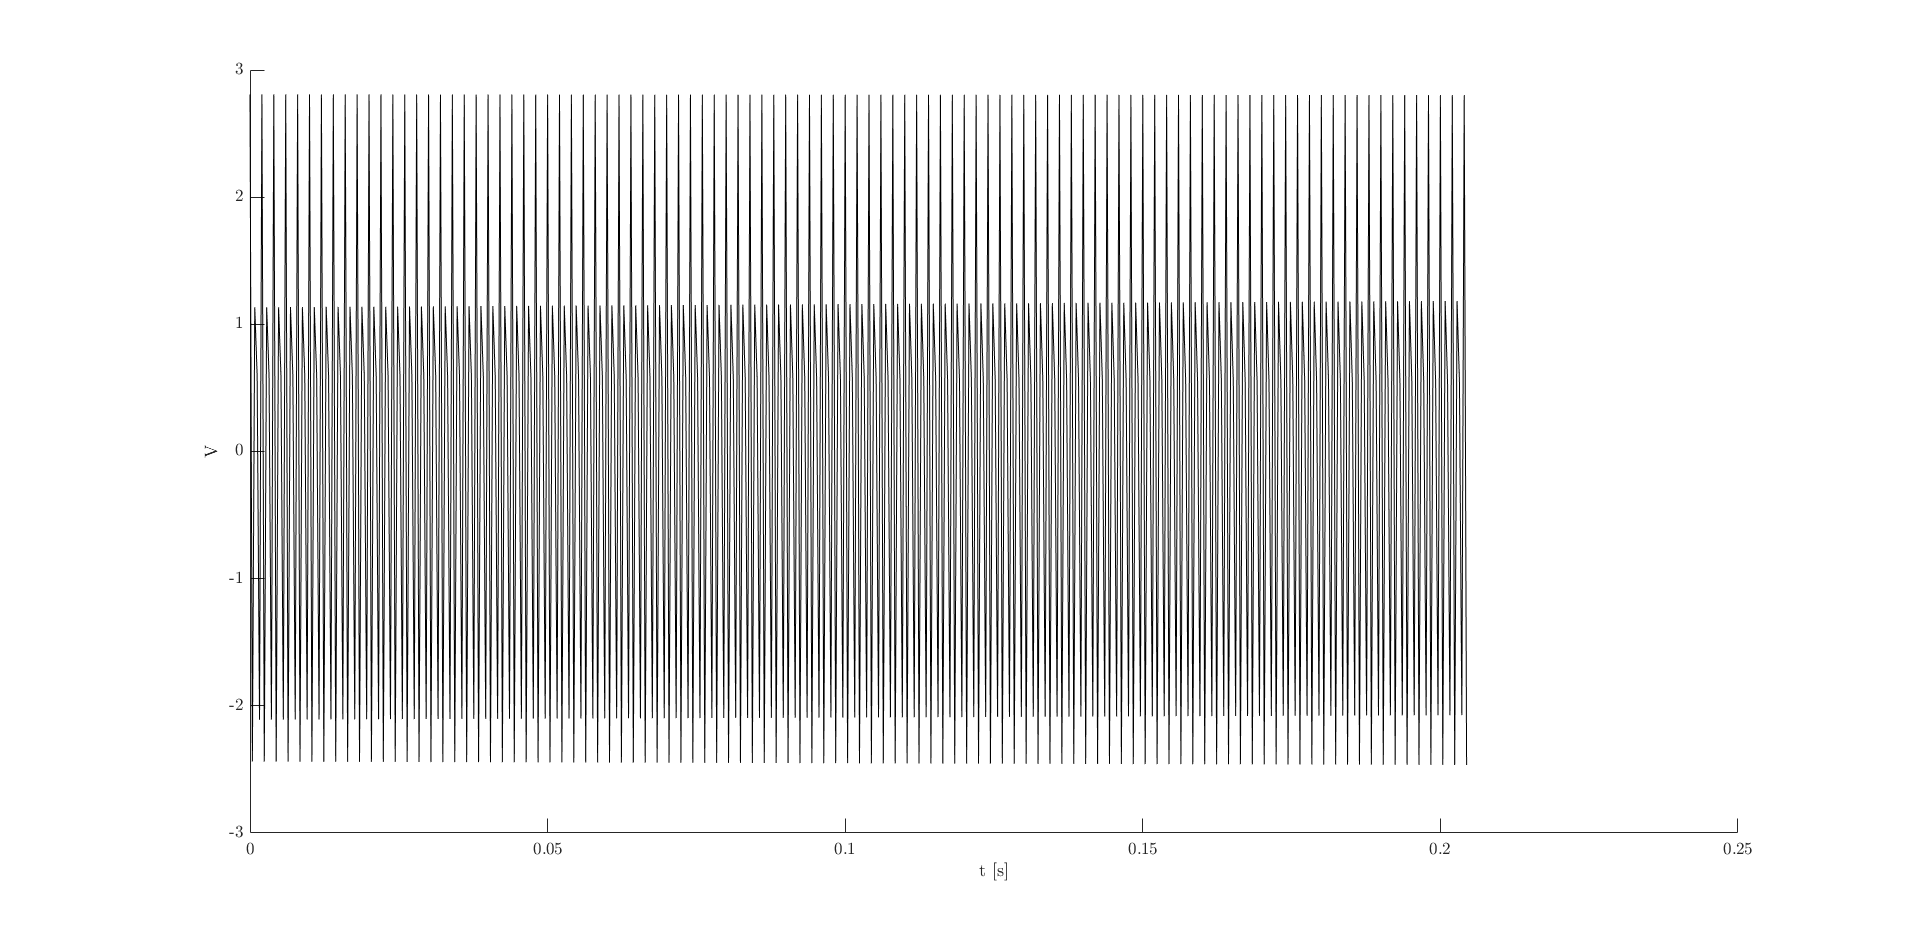
\includegraphics[width=.28\linewidth]{sineTime2500.png}
\label{fs>f}}
\quad
\subfigure[$f_s\ = \ f$]{
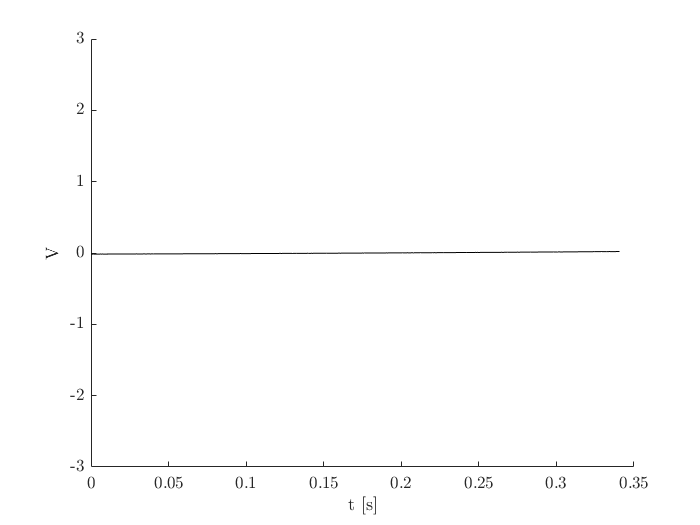
\includegraphics[width=.28\linewidth]{sineTime1500.png}
\label{fs=f}}
\quad
\subfigure[$f_s\ < \ f$]{
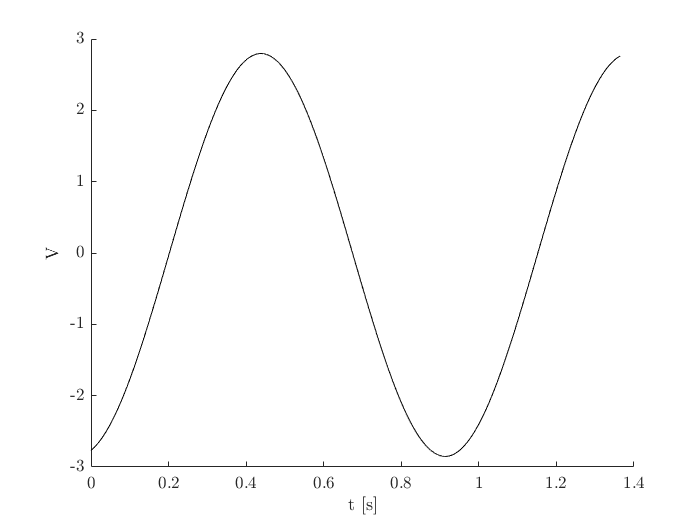
\includegraphics[width = .28\linewidth]{sineTime1501.png}
\label{fs<f}}
\caption{Sine and square waves with $V_{rms}$ of 2V at 100Hz shown in the frequency domain}
\label{TimeDomainImages}
\end{figure}

Analysis of known signals in the time domain also qualitatively matched theoretical predictions. From Figure \ref{fs>f}, it is shown that the observable frequency is equivalent to the signal via the function generator. The shape and amplitude, however, cannot be recovered and is a consequence of the Nyquins frequency being insufficient to properly measure the incoming signal. When adjusting the sampling rate to match the signal frequency, it is shown in Figure \ref{fs=f} that the time trace will consist of a straight line. This phenomenon was due to the NI-DAQ measuring the same point on the curve every cycle and, in this experiment, the measured point also aligned to the point where the amplitude of the sine wave was equal to zero. Adjusting the signal frequency such that $f_s < f $, however, did not align with the anticipated results in the time domain. The anticipated result was a time trace with no particular shape, amplitude, nor frequency but the results shown in Figure \ref{fs<f} shows an entirely different outcome. Experimental data shows a sinusoidal wave with a frequency of approximately 1 Hz.  

\subsection{Analysis of Unknown Signal}

% :::::::::::::::::: Mystery Wave Subsection ::::::::::::::::::
Plotting the time trace for the unknown signal revealed a high frequency component embedded in a low frequency signal.

\begin{figure}[ht]
    \centering
    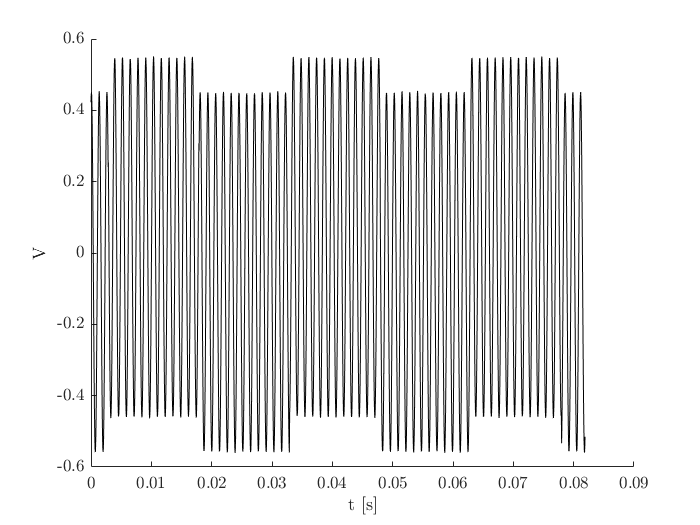
\includegraphics[width = .4\linewidth]{mysteryTime.png}
    \caption{Time trace of unknown signal}
    \label{UnknownTime}
\end{figure}

The power spectra of the unknown signal was examined at sampling frequencies of 1 kHz and 2 kHz. Comparing the two samples reveals that the former of the sampling frequencies aliased the signal and is most apparent by the shift in the largest peek.

\begin{figure}[ht]
\centering
\subfigure[$f_s$ = 1 kHz]{
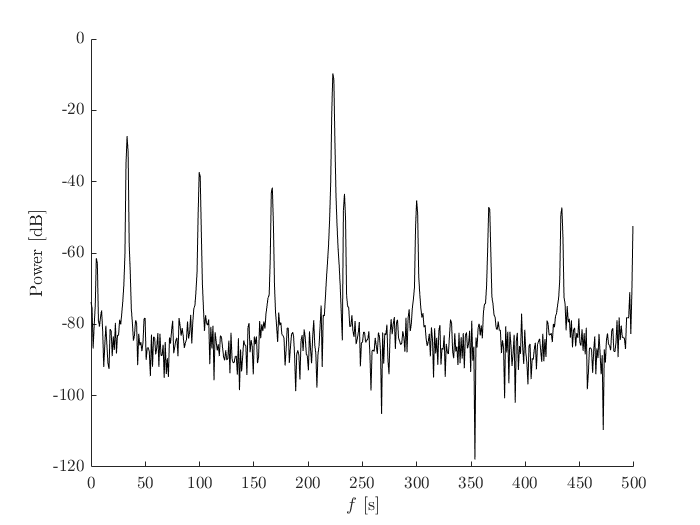
\includegraphics[width=.4\linewidth]{mystery1000.png}
\label{Unknown1khz}}
\quad
\subfigure[$f_s$ = 2 kHz]{
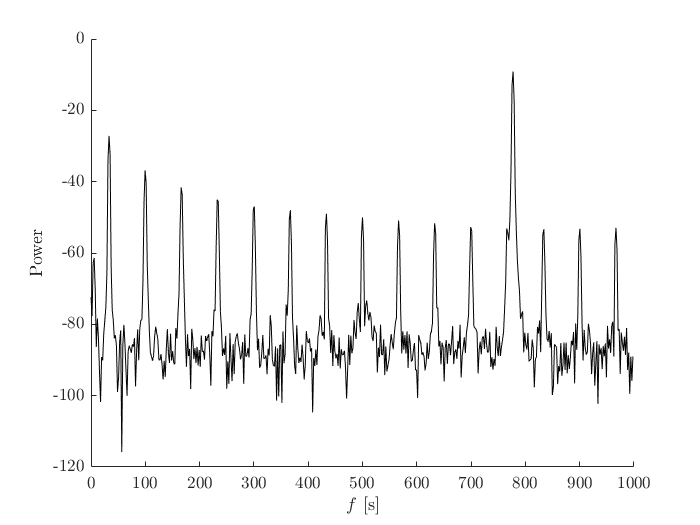
\includegraphics[width=.4\linewidth]{mystery2000.png}
\label{Unknown2khz}}
\caption{Power Spectrum for unknown signal}
\label{UnknownSignalFigures}
\end{figure}

 Further investigation of the power spectra confirmed the existence of a low frequency signal with harmonics (i.e., square or triangle wave) and a high frequency signal with no harmonics (i.e., sinusoidal wave). The \emph{fold back} behavior shown by comparing Figures \ref{Unknown1khz} and \ref{Unknown2khz} is representative of a wave at 777Hz and being aliased using a 1 kHz sampling rate. In Figure \ref{Unknown1khz}, the observed frequency of the sine wave occurs at 223 Hz $\pm$ df and this observation matches the theoretical outcome described in Equation \ref{fobsEq}.

The harmonics observed in the unknown signal matched to known signals via trial and error but based on the assumption that the underlying wave was either a square or triangle wave. Figure \ref{GuessActual} shows the measured signal in blue and a replicated signal in black. The replicated signal was created using the function generated and combining two sets of data. The first set of data was obtained by creating a sine wave with a frequency of 777 Hz and the second data set was obtained by generating a triangle wave at 33 Hz and 50\% symmetry. A side by side qualitatively shows that replicated signal matches harmonic frequency of the unknown signal. The amplitude of the signals, however, differed in magnitude since the replicated signal carried more energy than the unknown signal. Table \ref{unknownSignalTable} showcases the frequencies associated with each graph, along with associated uncertainties.

\begin{figure}[ht]
    \centering
    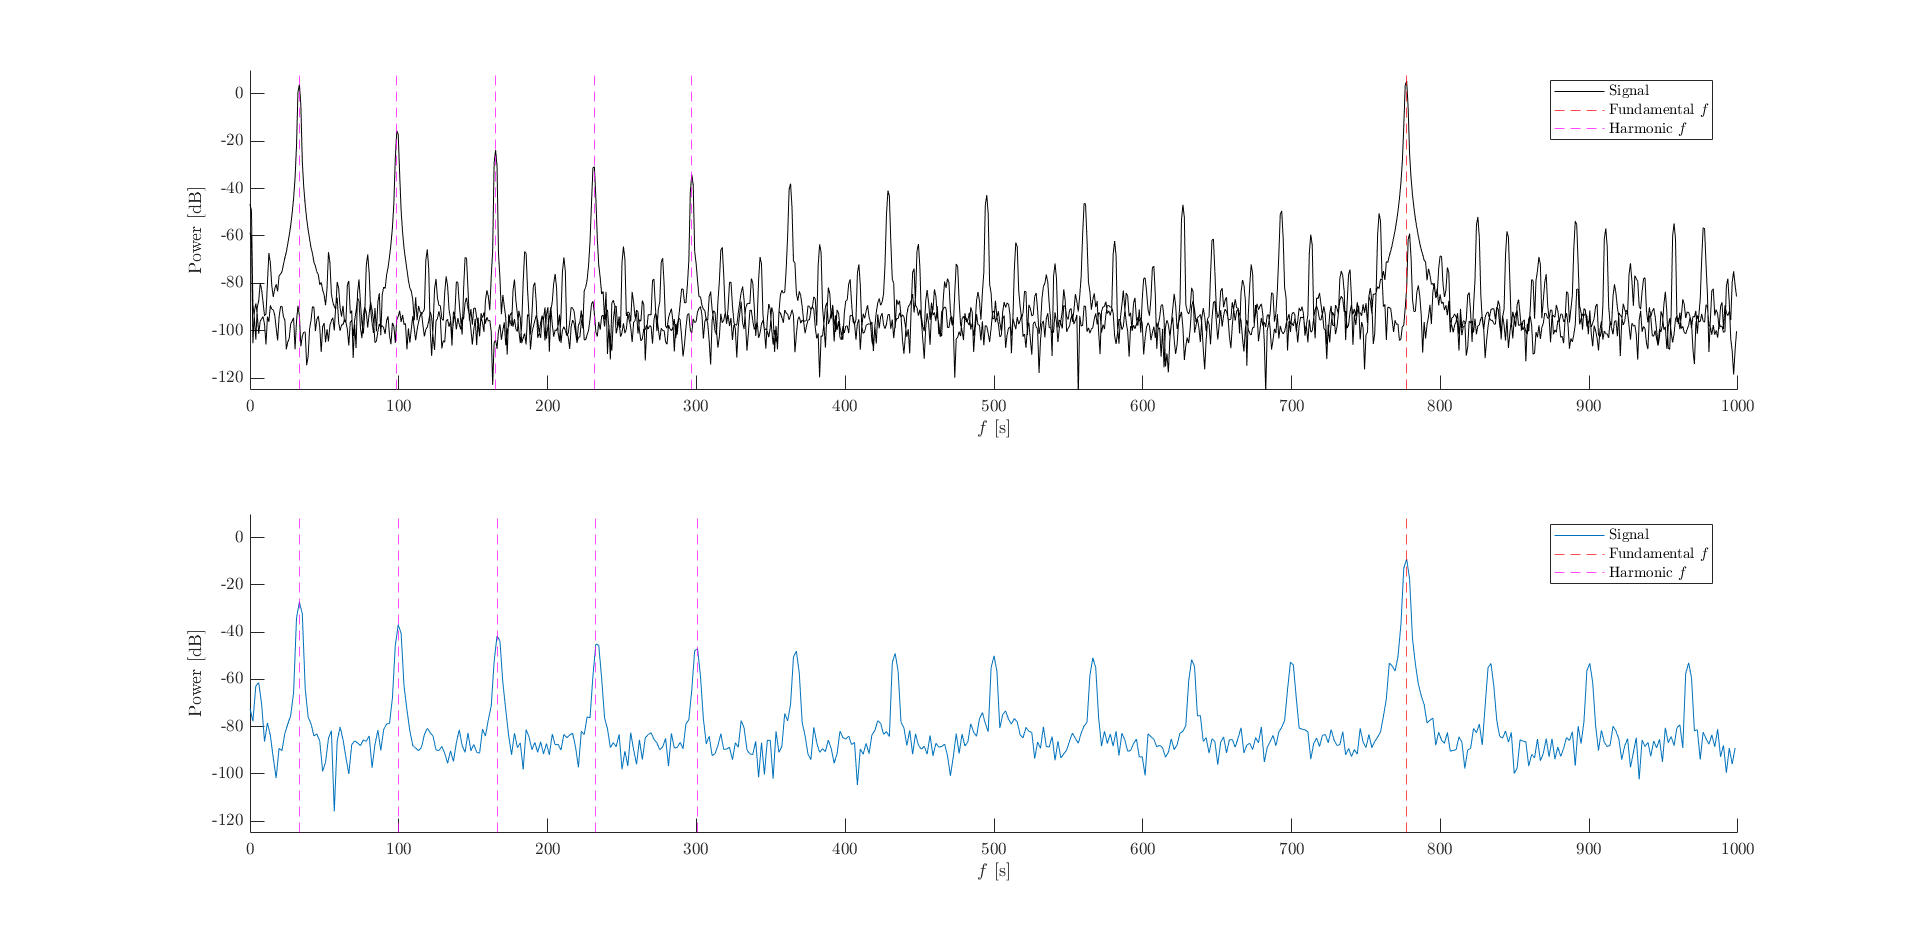
\includegraphics[width=.8\linewidth]{mysteryLab.png}
    \caption{Guess and Actual}
    \label{GuessActual}
\end{figure}

\begin{table}[ht]
    \centering
    \begin{tabular}{c|c||c|c|c|c}
         & Sine $f$ & Triangle $f$ & Triangle $f_3$ & Triangle $f_5$ & Triangle $f_7$ \\ \hline
         $f_{unk}$ [Hz] & 777  & 33  & 100 & 166 & 232\\ \hline
         $f_{rep}$ [Hz] & 777  & 33  & 99  & 165 & 231\\ \hline
    \end{tabular}
    \caption{Caption}
    \label{unknownSignalTable}
\end{table}

\section{Conclusion}
Representing signals in the frequency domain is an efficient method for managing large sets of data. Rather representing a signal with a relatively large set of data points, a signal can be represented with a by a fundamental frequency and, if applicable, a series of harmonic frequencies. Additionally, analyzing unknown frequencies in the power spectrum provides a simplified approach to identifying various types of waves embedded in a signal.

\newpage
\appendix

\section{MATLAB Script}
\lstinputlisting[style=Matlab-editor]{lab7.m}


\end{document}